%for a more compact document, add the option openany to avoid
%starting all chapters on odd numbered pages
\documentclass[12pt]{cmuthesis}

% This is a template for a CMU thesis.  It is 18 pages without any content :-)
% The source for this is pulled from a variety of sources and people.
% Here's a partial list of people who may or may have not contributed:
%
%        bnoble   = Brian Noble
%        caruana  = Rich Caruana
%        colohan  = Chris Colohan
%        comar    = Cyrus Omar
%        jab      = Justin Boyan
%        josullvn = Joseph O'Sullivan
%        jrs      = Jonathan Shewchuk
%        kosak    = Corey Kosak
%        mjz      = Matt Zekauskas (mattz@cs)
%        pdinda   = Peter Dinda
%        pfr      = Patrick Riley
%        dkoes = David Koes (me)

% My main contribution is putting everything into a single class files and small
% template since I prefer this to some complicated sprawling directory tree with
% makefiles.

% some useful packages
\usepackage[charter]{mathdesign}
\usepackage{fullpage}
\usepackage{graphicx}
\usepackage{amsmath}
\usepackage[numbers,sort]{natbib}
\usepackage[backref,pageanchor=true,plainpages=false, pdfpagelabels, bookmarks,bookmarksnumbered,
%pdfborder=0 0 0,  %removes outlines around hyper links in online display
]{hyperref}
\usepackage{subfigure}

% Approximately 1" margins, more space on binding side
%\usepackage[letterpaper,twoside,vscale=.8,hscale=.75,nomarginpar]{geometry}
%for general printing (not binding)
\usepackage[letterpaper,twoside,vscale=.8,hscale=.75,nomarginpar,hmarginratio=1:1]{geometry}

% Provides a draft mark at the top of the document. 
\draftstamp{\today}{DRAFT}

\begin {document} 
\frontmatter

%initialize page style, so contents come out right (see bot) -mjz
\pagestyle{empty}

\title{ %% {\it \huge Thesis Proposal}\\
{\bf Practical Concurrency Testing} \\
\normalsize \vspace{1em}
{\em or, How I Learned to Stop Worrying and Love the Exponential Explosion}}
\author{Ben Blum}
\date{Decembruary 2018}
\Year{2018}
\trnumber{}

\committee{
Garth Gibson, Chair \\
David A. Eckhardt \\
Brandon Lucia \\
Haryadi Gunawi, University of Chicago
}

\support{}
\disclaimer{}

% copyright notice generated automatically from Year and author.
% permission added if \permission{} given.

\keywords{landslide terminal, baggage claim, ground transportation, ticketing}

\maketitle

\begin{dedication}
For Elsie, Margie, Johnny, Mel, Eve, and David, who brought me here today.
\end{dedication}

\pagestyle{plain} % for toc, was empty

%% Obviously, it's probably a good idea to break the various sections of your thesis
%% into different files and input them into this file...

\begin{abstract}
Concurrent programming presents a challenge to students and experts alike because of the complexity of multithreaded interactions and the difficulty to reproduce and reason about bugs.
Stateless model checking is a concurrency testing approach which forces a program to interleave its threads in many different ways, checking for bugs each time.
This technique is powerful, in principle capable of finding any nondeterministic bug in finite time,
but suffers from exponential explosion as program size increases.
Checking an exponential number of thread interleavings is not a practical or predictable approach for programmers to find concurrency bugs before their project deadlines.

In this thesis, I develop several new techniques to make stateless model checking more practical for human use.
I have built Landslide, a stateless model checker specializing in undergraduate operating systems class projects.
Landslide extends the traditional model checking algorithm with a new framework for automatically managing
%the exploration of
multiple state spaces according to their estimated completion times,
which I show quickly finds bugs should they exist and also quickly verifies correctness otherwise.
I evaluate Landslide's suitability for inexpert use by presenting the results of many semesters providing it to students in 15-410, CMU's Operating System Design and Implementation class,
and more recently, students in the operating systems classes at the University of Chicago and Berkeley.
%Finally, I will present several new techniques that allow stateless model checking to be practically employed on real-world programs.
%Finally, I will explore broader impact by extending Landslide to test some real-world programs and to be used by students at other universities.
Finally, I extend Landslide with a new concurrency model for hardware transactional memory,
and evaluate several real-world transactional benchmarks to show that stateless model checking can keep up with the developing concurrency demands of real-world programs.
\end{abstract}

\begin{acknowledgments}
I thank the online Android: Netrunner community Stimhack.
\\

Please hold on. This thesis will be departing shortly for the Landslide terminal, baggage claim, ground transportation, and ticketing.
\end{acknowledgments}

\newpage
\begin{figure}[h]
	\vspace{12em}
	\begin{center}
		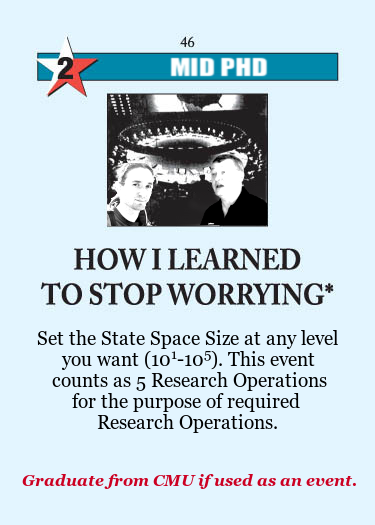
\includegraphics[width=0.5\textwidth]{how-i-learned.png}
	\end{center}
\end{figure}


\tableofcontents
\listoffigures
\listoftables

\mainmatter

%% Double space document for easy review:
%\renewcommand{\baselinestretch}{1.66}\normalsize

% The other requirements Catherine has:
%
%  - avoid large margins.  She wants the thesis to use fewer pages, 
%    especially if it requires colour printing.
%
%  - The thesis should be formatted for double-sided printing.  This
%    means that all chapters, acknowledgements, table of contents, etc.
%    should start on odd numbered (right facing) pages.
%
%  - You need to use the department standard tech report title page.  I
%    have tried to ensure that the title page here conforms to this
%    standard.
%
%  - Use a nice serif font, such as Times Roman.  Sans serif looks bad.
%
% Other than that, just make it look good...

\newcommand{\inspirationallinebreak}{\vspace{0.25em}}
\newcommand\inspirationalquote[2]{\begin{flushright}
	\vspace{-1em}
	\fontfamily{pzc}\selectfont
	{\em #1}
	\inspirationallinebreak

	---{#2}
	\fontfamily{mdbch}\selectfont
	\vspace{2em}
\end{flushright}}

\chapter{Introduction}

\chapter{Background}

\chapter{410} % rename
\inspirationalquote{Knowing the students might one day
%find a way to
fix their concurrency bugs...
it fills you with determination.}{Undertale (paraphrased)}

\chapter{Related Work}
\inspirationalquote{I see now that none of us are yet ready. The cycle exists so that we may
improve ourselves. But \\
the one who reaches the summit is not our superior, for
they stand on our shoulders to reach it.}
{The Shepherd v82.6.0174, The Talos Principle}


\chapter{Conclusion}
\inspirationalquote{
%	``If you are a god, Zeus, as the stories claim, then why did you create evolution?
%	Why did you make \\ a world that can only grow through cruelty and pain?''
%	\inspirationallinebreak
%
%For a moment--surely this meant death was near--she thought she heard him answer:
%``My child, I \\
%was shaped by the gods that came before me, as you were shaped by me.
%The choice I had was be- \\
%tween creation and oblivion, life and death.
%And I chose life, because any life is better than no life, \\
%because as long as there is life, there is hope--if not for us, then for some generation to come.''
%	\inspirationallinebreak
%
%``Then how are you a god, if you can offer so little?'' she whispered, feeling death creep closer.
%	\inspirationallinebreak
%
%``I am a god because I take upon myself the burden of creation,'' the statue replied.
%	\inspirationallinebreak
%
%``Then we are all gods,'' Alexandra said, and pushed the button.}
	\begin{tabular}{p{0.875\textwidth}}
	``If you are a god, Zeus, as the stories claim, then why did you create evolution?
	Why did you make a world that can only grow through cruelty and pain?''
	\\
	For a moment--surely this meant death was near--she thought she heard him answer:
	``My child, I was shaped by the gods that came before me, as you were shaped by me.
	The choice I had was between creation and oblivion, life and death.
	And I chose life, because any life is better than no life,
	because as long as there is life, there is hope--if not for us, then for some generation to come.''
	\\
	``Then how are you a god, if you can offer so little?'' she whispered, feeling death creep closer.
	\\
	``I am a god because I take upon myself the burden of creation,'' the statue replied.
	\\
	``Then we are all gods,'' Alexandra said, and pushed the button.
	\end{tabular}}
{The Talos Principle (Road to Gehenna)}

asdfasdasdf
%\appendix
%\include{appendix}

\backmatter

%\renewcommand{\baselinestretch}{1.0}\normalsize

% By default \bibsection is \chapter*, but we really want this to show
% up in the table of contents and pdf bookmarks.
\renewcommand{\bibsection}{\chapter{\bibname}
\inspirationalquote{Only a doctor of philosophy, Darth.}{Robert Marsh, via Twitter}
}
%\renewcommand{\bibpreamble}{This text goes between the ``Bibliography''
%  header and the actual list of references}
\bibliographystyle{plainnat} % plain n'at
\bibliography{register} %your bib file

\end{document}
